

\chapter{Podstawowe definicje i założenia}
W niniejszym rozdziale przedstawiam podstawowe definicje, niezbędne do dalszych
rozważań.

W całej pracy jako pierścień będziemy rozumieć pierścień z jedynką.

\section{Definicja algebry z dzieleniem}
Definicję algebry przedstawiam za \cite{opial}.
\begin{definicja}
 \textit{Algebrą} nad ciałem $K$ nazywamy strukturę $(K,+,\cdot,0,
1;V,+,\cdot,\mathbb{0},\mathbb{1};\cdot )$ spełniającą następujące warunki:
\begin{enumerate}
 \item $V$ jest pierścieniem ze względu na określone w nim dwa działania
wewnętrzne - dodawanie $+$ i mnożenie $\cdot$
 \item zbiór $V$ jest przestrzenią liniową nad ciałem $K$ ze względu na
dodawanie i mnożenie zewnętrzne elementów zbioru $V$ przez elementy ciała $K$
 \item dla dowolnych elementów $v$,$w$ zbioru $V$ i dowolnego elementu $\alpha$
z ciała $K$ zachodzi: 
\begin{equation}
(\alpha \cdot v) \cdot w=v \cdot (\alpha \cdot w)=\alpha \cdot (v \cdot w) 
\label{warunek:pslacznosc}
\end{equation}
\end{enumerate}
\end{definicja}
Działania oznaczone przez $\cdot$ rozumiemy jako trzy różne działania: mnożenie
w ciele $K$, mnożenie zewnętrzne wektora ze zbioru $V$ przez element ciała $K$ i
mnożenie wewnętrzne w zbiorze $V$, jak to zostało przyjęte zwyczajowo, w
zapisie pomijamy. Zapis taki nie powinien prowadzić do nieporozumień.

Jeśli zażądamy by $(V,+,\cdot,\mathbb{0},\mathbb{1})$ był pierścieniem z
dzieleniem, otrzymaną strukturę nazywać będę algebrą z dzieleniem. Dokładniej
\begin{definicja}
 Algebrą z dzieleniem nazywać będę strukturę
$(K,+,\cdot,0,1;V,+,\cdot,\mathbb{0},\mathbb{1};\cdot )$ spełniającą wszystkie
warunki
definicji algebry i dodatkowo dla każdego niezerowego elementu $w$ ze zbioru $V$
istnieje
element odwrotny $v$ 
\begin{equation}
\forall_{w\in V \backslash \left\lbrace \mathbb{0} \right\rbrace } \,
\exists_{v\in V} \quad 
wv=vw=\mathbb{1}.
\label{warunek:elementodwrotny}
\end{equation}
Element $v$ nazywać będę elementem odwrotnym do elementu $w$ i oznaczać przez
$w^{-1}$.
\end{definicja}

\begin{przyklad}
Jeżeli przyjmiemy $V=K^3$ i rozważymy mnożenie $\cdot : V \times V
\longrightarrow V$ takie, że dla $v=\left[ 
\begin{array}{l}
a_1\\
a_2\\
a_3
\end{array} \right] 
$ i $w=\left[ 
\begin{array}{l}
b_1\\
b_2\\
b_3
\end{array} \right]$ 
$$v \cdot w = \left[ 
\begin{array}{l}
a_{2}b_{3} - a_{3}b_{2}\\
a_{3}b_{1} - a_{1}b_{3}\\
a_{1}b_{2} - a_{2}b_{1}
\end{array} \right], $$
to V jest algebrą. Działanie $\cdot$ jest zwane mnożeniem wektorowym.
\label{przyk:algebra}
\end{przyklad}
Struktura przedstawiona w przykładzie \ref{przyk:algebra} nie jest natomiast
algebrą z dzieleniem, gdyż nie spełnia warunku \ref{warunek:elementodwrotny}.

\begin{przyklad}
Przestrzeń macierzy nieosobliwych $M_{n \times n}\left( \mathbb{R} \right)$ z
mnożeniem i dodawaniem macierzy jest algebrą z dzieleniem, dla ustalonego $n$. 
\end{przyklad}

Przy rozważaniach algebry z dzieleniem ciekawą strukturą okazuje się algebra
kwaternionów Hamiltona.

\begin{definicja}
 Algebrą kwaternionów nazywamy zbiór
$\mathbb{H}=\mathbb{C}+\mathbb{C}j=\mathbb{R}+\mathbb{R}i+\mathbb{R}j+\mathbb{R}
k
$ z mnożeniem realizowanym według zasad:
\begin{equation}
i^2=j^2=k^2=-1
\end{equation}
\begin{eqnarray}
ij=k & jk=i & ki=j \\
ji=-k & kj=-i & ik=-j 
\end{eqnarray}
\end{definicja}
%Twierdzenie że H jest algebrą z dzieleniem.
Możemy rozważyć też ogólniejszą strukturę kwaternionów Hamiltona.
\begin{definicja}
 Dla ustalonych niezerowych $a,b\in K$ uogólnioną algebrą kwaternionów nad
$K$ nazywamy zbiór
$A=K+Ki+Kj+Kk$ z mnożeniem o elemencie neutralnym $\mathbb{1}=1$ realizowanym
według zasad:
%\begin{equation}
%i^2=j^2=k^2=-1
%\end{equation}
\begin{eqnarray} 
i^2=a & j^2=b & k^2=-ab \\
ij=k & jk=i & ki=j \\
ji=-k & kj=-i & ik=-j 
\end{eqnarray}
i oznaczymy go przez $\left(\frac{a,b}{K}\right) $
\end{definicja}
Jak łatwo zauważyć $\left(\frac{-1,-1}{\mathbb{R}}\right) = \mathbb{H}$.
\begin{definicja}
  Dla $x \in A$, $x=c_0+c_1i+c_2j+c_3k$, sprzężeniem $x$ nazwiemy 
\begin{equation}
\overline{x}=c_0-c_1i-c_2j-c_3k
\end{equation}
\end{definicja}

\begin{definicja}
  Dla $x \in A$, $x=c_0+c_1i+c_2j+c_3k$, normą $x$ nazwiemy wartość
\begin{equation}
\left\|x \right\| =x\overline{x}=c_0^2-ac_1^2-bc_2^2 +abc_3^2
\end{equation}
\end{definicja}

\begin{wlasnosci}
 Dla $x,y \in A$, $x=c_0+c_1i+c_2j+c_3k$, zachodzi:
\begin{enumerate}
\item $\overline{x+y}=\overline{x}+\overline{y}$
\item $\overline{ \left( xy \right) }=\overline{y} \, \overline{x}$
\item $\left\|xy \right\| =\left\|x \right\| \left\|y \right\|$
\item $\left\| \overline{x} \right\|=\left\|x \right\|  =x\overline{x}$
\end{enumerate}
\end{wlasnosci}

Odnośnie kwaternionów Hamiltona wiemy, że spełniają one warunki algebry z
dzieleniem. Nasuwa się zatem pytanie: czy uogólniona algebra kwaternionów jest
algebrą z dzieleniem? Okazuje się, że nie zawsze.

\begin{twierdzenie}
 Dla $A=\left(\frac{a,b}{K}\right) $, następujące warunki są prawdziwe:
\begin{enumerate}
 \item $A$ jest algebrą z dzieleniem
 \item $x\in A- \left\lbrace \mathbb{0} \right\rbrace \Rightarrow \left\|
x\right\| \neq 0 $
 \item $\forall (c_0,c_1,c_2)\in K : c_0^2=ac_1^2+bc_2^2 \Rightarrow
c_0=c_1=c_2=0$.
\end{enumerate}
\end{twierdzenie}
\begin{proof}
 tutaj będzie sobie dowód
co należało wykazać.
\end{proof}











\newpage
\begin{figure}[h]
\centering
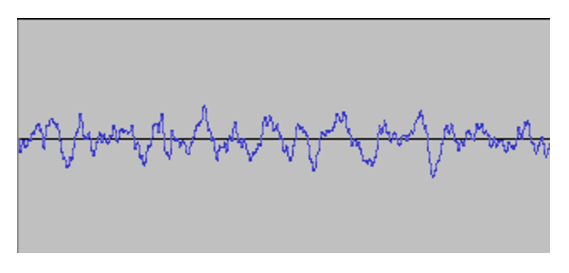
\includegraphics[scale=0.8]{grafika/signal} %plik grafiki
\caption[Przykładowy wykres sygnału dźwiękowego]{Przykładowy sygnał
dźwiękowy (wygenerowane przy pomocy programu Audacity)}
\label{fig:sygnal}
\end{figure}
Dźwięk rozumiany jako fala akustyczna opisuje się za pomocą widma. Widmo
jest funkcją $P$ od częstotliwości $f$, której wartość oznacza natężenie
składowej (rys. \ref{fig:spectra}).
\begin{figure}[h]
\centering
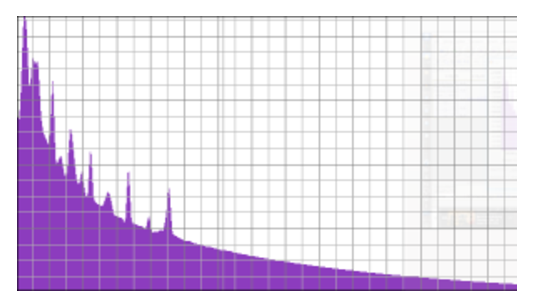
\includegraphics[scale=0.8]{grafika/widmo}
\caption[Przykładowy wykres widma]{Przykładowe widmo
dźwięku (wygenerowane przy pomocy programu Audacity)}
\label{fig:spectra}
\end{figure}

Dźwięki wywołują szereg wrażeń, które możemy opisać cechami
fizycznymi. Do najbardziej podstawowych wrażeń zaliczamy głośność, wysokość oraz
barwę. Głośność jest związana z natężeniem dźwięku (amplitudą drgań). Wysokość
określa wrażenie wywołane dźwiękiem o podanej częstotliwości 
\cite{zarysoMuzyce}.

Barwa jest subiektywną cechą, która pozwala rozróżnić dźwięki różniące się
charakterem i jakością. Jest zależna od widma. Pozwala odróżnić instrumenty
użyte do wydobycia dźwięku oraz różne głosy ludzkie \cite{zarysoMuzyce}. Dlatego
analiza barwy dźwięku jest stosowana przy
rozpoznawaniu mowy \cite{rozdzialQBH_MFCC}.

\section{Współczynniki ceptralne w skali Mel}
Algorytmy sprawdzające się przy obliczaniu podobieństwa utworów muzycznych
bazują na analizie widma dźwięku. Do tego zagadnienia wykorzystuje się ceptralne
współczynniki w skali Mel (ang. \textit{Mel Frequency Ceptral Coefficients}). Są
to wartości
liczbowe opisujące cechy widma dźwięku na niewielkim przedziale czasu. Kroki
algorytmu ich wydobycia z dźwięku jednokanałowego (jeśli zachodzi taka
potrzeba, utwór jest konwertowany na jednokanałowy) 
%(rys. \ref{fig:tracksignal}) 
są następujące \cite{magisterska}:

%\begin{figure}[h]
%\centering
%\includegraphics[scale=0.25]{grafika/tracksignal} %plik grafiki
%\caption[Sygnał utworu]{Sygnał dźwiękowy utworu\newline (wygenerowane przy
%pomocy programu sound2png pakietu MARSYAS)}
%\label{fig:tracksignal}
%\end{figure}
\begin{enumerate}
 \item Sygnał $x(t)$ jest dzielony na ramki, zazwyczaj po około 20-25ms.
 \item Na każdą ramkę nakłada się funkcję okna (najczęściej Hamminga
lub Hanna).
 \item Następnie jest stosowana dyskretna transformata Fouriera (DFT) dla każdej
ramki, w wyniku czego otrzymuje się widmo dźwięku $P(f)$ %(rys.
.%\ref{fig:trackspectrum})

%\begin{figure}[h]
%\centering
%\includegraphics[scale=0.5]{grafika/trackspectrum} %plik grafiki
%\caption[Widmo utworu]{Widmo utworu\newline (wygenerowane przy pomocy programu
%sound2png pakietu MARSYAS)}
%\label{fig:trackspectrum}
%\end{figure}
 \item Widmo $P(f)$ jest skalowane względem osi częstotliwości $f$ do
reprezentacji Mel według wzoru
\begin{equation}
 M(f)=2596\log_{10}\left(1+\frac{f}{700}\right) ,
\end{equation} 
która dobrze odzwierciedla ludzkie postrzeganie dźwięku.
 \item Silnie skorelowane wartości Mel są redukowane przez zastosowanie
dyskretnej transformaty kosinusowej (DCT). W wyniku tego otrzymujemy $N$ cech
dla każdej ramki czasowej.
\end{enumerate}
Różne algorytmy ustalają przyjętą na początku szerokość ramki, czas
próbkowania sygnału, liczbę wydobytych współczynników oraz wiele innych założeń.

Wydobycie współczynników MFCC dla całego utworu muzycznego trwa stosunkowo
długo. Przy implementacji programu wykorzystywano pakiet MARSYAS do
analizy sygnału i wydobycia potrzebnych danych z pliku utworu. 

\section{Wielowymiarowy model Gaussa}
Rozkładem $n$-wymiarowym normalnym (Gaussa) \cite{Gaussa} nazywamy rozkład
prawdopodobieństwa
$n$-wymiarowego wektora losowego $X=\left[ X_1, X_2,\ldots , X_n \right] ^T $ o
funkcji gęstości określonej wzorem
\begin{equation}
f(x)=\frac{1}{\sqrt{(2\pi )^n \left| \Sigma \right| }}\exp
\left( -\frac{1}{2} (x-\mu )^{T}\Sigma ^{-1} (x-\mu ) \right) 
\end{equation}
gdzie $\mu= E(X)$ jest wektorem wartości oczekiwanych, a $\Sigma=E[(x-\mu
)(x-\mu )^T]$. W szczególności zachodzi
\begin{equation} \Sigma=\left[ 
\begin{array}{cccc}
cov(X_1,X_1) & cov(X_1,X_2) & \ldots & cov(X_1,X_n)\\
cov(X_2,X_1) & cov(X_2,X_2) & \ldots & cov(X_2,X_n)\\
\vdots & \vdots & \ddots & \vdots\\
cov(X_n,X_1) & cov(X_n,X_2) & \ldots & cov(X_n,X_n)
          \end{array} \right]
\end{equation}
przy czym
\begin{equation}
cov(X_i, X_j)=E(X_i X_j) - E(X_i) E(X_j).
\end{equation}

Przy modelowaniu danych, wektor $\mu$ należy interpretować jako środek skupiska
badanych danych. Natomiast macierz kowariancji $\Sigma$ opisuje rozrzut danych
na około tego środka w różnych kierunkach.

\section{Koncepcje algorytmów}
Międzynarodowe towarzystwo naukowe zajmujące się eksploracją informacji z
muzyki \textit{International Society for Music Information Retrivial} (ISMIR) co
roku organizuje konkurs, w którym konkurują różne implementacje systemów
służących między innymi do wyznaczania podobieństwa utworów muzycznych. Dzięki
tym konkursom algorytmy określające podobieństwo lub
stwierdzające do jakiego gatunku muzycznego należy utwór reprezentują wysoki
poziom w zakresie skuteczności działania.

Metody wyznaczania podobieństwa muzyki, związane z nazwiskami twórców
algorytmów, na które warto zwrócić uwagę są następujące \cite{magisterska}:
\begin{description}
 \item[Beth Logan i Ariel Salomon (LS)] Algorytm bazuje na klastrowaniu wektorów
współczynników MFCC metodą $k$-średnich i przechowywaniu danych na temat
wszystkich skupisk w postaci średniej, macierzy kowariancji oraz wagi skupiska.
W fazie porównywania utworów wykorzystuje się Earth Movers Distance oraz
symetryzowaną dywergencję Kullbacka-Leiblera.
 \item[Jean-Julien Aucountier i Francois Pachet (AP)] Algorytm opiera się na
podzieleniu wektorów współczynników MFCC na trzy skupiska metodą
\textit{Expectation Maximisation}, które opisuje się dalej mieszanymi modelami
Gaussa (\textit{Gaussian mixture models}). W fazie porównywania utworów
wyliczane jest prawdopodobieństwo nakładania się dwóch modeli metodą Monte
Carlo.
 \item[Michael Mandel i Dan Ellis (ME)] Algorytm ten opiera się na wyliczeniu
modelu Gaussa opisującego wszystkie wektory MFCC dla utworu. Natomiast w fazie
porównywania utworów wyliczana jest zsymetryzowana dywergencja
Kullbacka-Leiblera.
 \item[Elias Pampalk, Andreas Rauber i Dieter Merkl (PRM)] Algorytm wykorzystuje
analizę rytmu.
 \item[Arthur Flexer, Elias Pampalk i Gerhard Widmer (FPW)] Algorytm korzysta z
ukrytych modeli Markova.
\end{description}

\section{Wybrany algorytm}
W niniejszej pracy zaimplementowano algorytm bazujący na pomyśle algorytmu
autorstwa Michael Mandel i Dan Ellis.
Stworzony algorytm jest szybki i nieskomplikowany, a jednocześnie
wystarczająco efektywny.

Model opisujący utwór zakłada, że dane wektory współczynników MFCC rozkładają
się zgodnie z wielowymiarowym rozkładem Gaussa.

Algorytm składa się z dwóch operacji: opisanie za pomocą modelu
matematycznego utworu muzycznego oraz generowanie listy odtwarzania. Konstrukcja
modelu realizowana jest w dwóch krokach:
\begin{enumerate}
 \item Wydobycie współczynników MFCC z utworu: po $n$ ($n=13$) wartości dla
każdej ramki.
 \item Wyznaczenie wektora kolumnowego średnich $\mu$ oraz
macierzy kowariancji $\Sigma$ 
dla $n$ ($n=13$) zmiennych opisujących estymowany rozkład Gaussa.
\end{enumerate}
Generowanie propozycji listy odtwarzania polega na wskazaniu przez algorytm $m$
($m=10$) propozycji utworów, najbardziej podobnych do wskazanego wcześniej
utworu:
\begin{enumerate}
 \item Pobranie modelu matematycznego wskazanego utworu.
 \item Dla wszystkich utworów w bazie danych jest liczona odległość uproszczoną
symetryzowaną dywergencją Kullbacka-Leiblera \cite{magisterska}
%d = trace(co1*ico2)+trace(co2*ico1)+trace((ico1+ico2)*(m1-m2)*(m1-m2)’)
\begin{equation}
\label{eq:KLdiv}
 d(u_1,u_2)=Tr(\Sigma_1 \times \Sigma_{2}^{-1})+Tr(\Sigma_2 \times
\Sigma_{1}^{ -1}) + Tr((\Sigma_{1}^{-1} + \Sigma_{2}^{-1}) \times (\mu_1 -
\mu_2) \times (\mu_2 - \mu_1)^{T})
\end{equation}
od wskazanego utworu i dodawana do listy rankingowej już przetworzonych utworów.
We wzorze (\ref{eq:KLdiv}) $Tr(M)$ oznacza ślad macierzy $M$ - sumę
$\sum_{i=0}^{n} m_{ii}$ wyrazów macierzy leżących na przekątnej, a $\times $ -
znak mnożenia macierzy.
 \item Zwracany jest wektor 10 utworów najbardziej podobnych według algorytmu.
\end{enumerate}

W literaturze proponowane są różne wariacje wskazanego algorytmu.
Wykorzystują różne wartości $n$ liczby współczynników MFCC. Tutaj użytych jest
$n=13$ współczynników wygenerowanych programem z pakietu MARSYAS.

Warto zauważyć, że przy obliczaniu odległości ze wzoru (\ref{eq:KLdiv})
wykonanie
pełnego mnożenia dwóch macierzy $\Sigma_1 \times \Sigma_{2}^{-1}$ jest zbędne.
Wystarczy wyliczyć wyrazy postaci $m_{ii}$ potrzebne do obliczenia śladu
macierzy, co skraca czas obliczeń.




